\documentclass[%
	%draft,
	%submission,
	%compressed,
	final, %technote,
	%internal,
	%submitted,
	%inpress,
	%reprint,
	% %titlepage,
	notitlepage,
	%anonymous,
	narroweqnarray,
	inline,
	twoside,
        %invited,
	]{ieee}

\usepackage[top=3cm, bottom=2cm, left=1.5cm, right=1.5cm,a4paper,includeheadfoot]{geometry}



\usepackage[utf8]{inputenc}			% idioma
\usepackage[spanish]{babel}
\usepackage{float}
%\usepackage{color}
%\usepackage{colortbl}
%\usepackage{amsmath}
%\usepackage{amsfonts}
%\usepackage{verbatim}

\usepackage{hyperref}				% urls

% -------- PARA FIGURAS
\usepackage{graphicx}
%\usepackage{capt-of}
% -------- FIN FIGURAS

% -------- PARA MONXTRAR EL CODIGO DE MANERA AMENA
\usepackage{courier}
\usepackage{listings}
\lstset{ %
	language=C++,                % choose the language of the code
	basicstyle=\footnotesize\ttfamily,       % the size of the fonts that are used for the code
	numbersep=5pt,                  % how far the line-numbers are from the code
%	backgroundcolor=\color{white},  % choose the background color. You must add \usepackage{color}
	showspaces=false,               % show spaces adding particular underscores
	showstringspaces=false,         % underline spaces within strings
	showtabs=false,                 % show tabs within strings adding particular underscores
	frame=single,           % adds a frame around the code
	tabsize=6,          % sets default tabsize to 2 spaces
	captionpos=b,           % sets the caption-position to bottom
	breaklines=true,        % sets automatic line breaking
	breakatwhitespace=false,    % sets if automatic breaks should only happen at whitespace
}
\usepackage{sidecap}
\usepackage{amsmath}
\usepackage{wrapfig}
\usepackage{caption}
\usepackage{subcaption}
\usepackage{tikz}
\usepackage{tikz-qtree}

\newcommand{\subsubsubsection}[1]{\paragraph{#1}\mbox{}\\}
\setcounter{secnumdepth}{4}
\setcounter{tocdepth}{4}
%\usepackage{minted}

%Formato de los links
\usepackage{hyperref}
\hypersetup{
  colorlinks   = true, %Colours links instead of ugly boxes
  urlcolor     = blue, %Colour for external hyperlinks
  linkcolor    = blue, %Colour of internal links
  citecolor   = red %Colour of citations
}
% -------- FIN CODIGO

\hypersetup{			%sacar los colores horrendos de las ref
	colorlinks=false,
	pdfborder={0 0 0},
}


\begin{document}


\title[Traceroute]{%
	Detección de Enlaces Intercontinentales
}

\author[COSTA, GATTI]{
\and{}Manuel Costa \authorinfo{M. Costa, e-mail: manucos94@gmail.com}%
\and{}Mathias Gatti\authorinfo{M. Gatti, e-mail: mathigatti@gmail.com}
}

%\journal{Grupo 13: Teor\'ia de las Comunicaciones, Departamento de Computaci\'on, UBA}

\firstpage{1}

\maketitle               

\begin{abstract} 
\end{abstract}

\begin{keywords}
traceroute, enlaces intercontinentales, ICMP, anomalías, RTT, TTL
\end{keywords}


\section{Introducción}

--- COMPLETAR ---

Iniciamos este trabajo con el objetivo de aprender sobre el protocolo ARP y más en general las redes de Internet y sus algoritmos de intercambio de paquetes.

A lo largo de este informe describiremos ciertos análisis que tendrán como objetivo el modelado de emisores de información y la posterior detección de símbolos destacados. A partir de esta metodología creemos que podremos identificar dispositivos claves en la red como por ejemplo el gateway. Nuestra hipótesis es que este tendrá destacará en el intercambio de paquetes who-has siendo de los que mas reciba y envíe.

--- COMPLETAR ---


\section{Métodos}

\subsection*{Herramientas}
Para la implementación de traceroute utilizamos el código provisto por la catedra al cual le realizamos ciertas modificaciones para poder detectar anomalías y guardar los datos obtenidos de forma más cómoda.

\subsection*{Detección de saltos intercontinentales}

Para la detección automática de saltos intercontinentales aplicamos una técnica basada en el Modified Thompson Tau Test para detección de outliers, como se explica en Cimbala\footnote{http://www.net.in.tum.de/fileadmin/TUM/NET/NET-2012-08-1/
NET-2012-08-1\_02.pdf}. Dicho test consiste en comparar el valor absoluto de las muestras estandarizadas (mediante z-score) contra un estadístico, $\tau$, que depende del tamaño de la muestra. En particular, nuestra versión difiere con la presentada con la de Cimbala en que no tomamos el valor absoluto del z-score, dado que no estamos interesados en detectar los casos atípicamente pequeños. 

\subsection*{Asunciones realizadas}
\begin{itemize}
	\item A los fines prácticos, vamos a considerar que un salto de América del Sur a América del Norte se considera un salto intercontinental, por la extensión del mismo.
	\item A veces se da el caso en que el RTT promedio para un cierto TTL puede ser menor que el RTT del TTL anterior. Ante esta situación seteamos el RTT diferencial (delta) en 0. Razones por las que puede suceder esto son el problema de los \emph{caminos asimétricos}, o bien que haya un desvío estándar elevado y el hop realizado sea corto. Se nos presento entonces la duda de si considerar estos valores o no a la hora de hacer el cálculo de los \emph{outliers}. Decidimos que tanto un problema como el otro pueden estar afectando a otros hops que sin embargo no llegaron a dar 0, pero dieron un valor menor al que deberían. Por lo tanto, sería injusto (y posiblemente un error metodológico) solo omitir a los valores nulos.
\end{itemize}


\subsubsection*{Rutas}
Se corrió traceroute sobre 3 universidades distintas con un ttl de 30 y 40 queries. Con el objetivo de lograr contrastar elegimos universidades muy lejanas y muy cercanas. A continuación describimos brevemente a cada una.

\begin{itemize}
	\item Universidad de São Paulo (www5.usp.br) esta será la universidad mas cercana, ubicada en el mismo continente, por lo cual esperamos que no haya ningún enlace intercontinental.
	\item Universidad de Sidney (www.sydney.edu.au) escogimos esta universidad ya que nos surgió la duda de si existirá algún enlace intercontinental directo entre oceanía y america o tendrá que pasar europa resultando en varios enlaces.
	\item Universidad de Moscú (www.msu.ru) al estar ubicada en un punto tan alejado de nosotros estabamos seguros de que iba a haber algún salto intercontinental y quizás más.
\end{itemize}

\section{Resultados y análisis}

\subsection*{Universidad de São Paulo}

\subsubsection*{Recorrido en el Planisferio}

A continuación se puede ver de forma bastante clara como el paquete tuvo que pasar por estados unidos para luego ir a Europa Occidental hasta llegar finalmente a Rusia.

\begin{figure}[H]
  \centering
  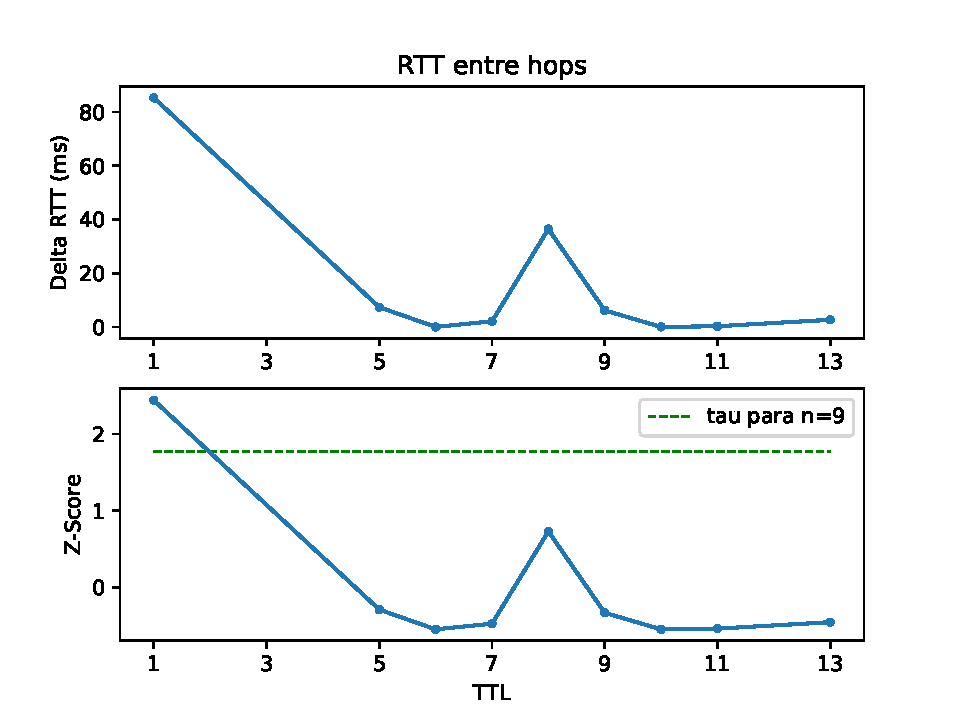
\includegraphics[width=8.5cm]{figs/traceroute-saopaulo.pdf}
  \caption{\normalfont Recorrido realizado por los paquetes durante la ejecución de traceroute al intentar alcanzar el sitio XXXXXXXXXXXXXXXXXXXXXXXXXX}
\end{figure}

\subsubsection*{RTT entre saltos}

A continuación intentamos ver los timepos entre saltos. Para esto calculamos la media de cada de los RTTs obtenidos de cada TTL para reducir a solo un valor las mediciones obtenidas por cada TTL. 

Seguido de esto realizamos dos experimentos. Primero simplemente restamos los RTTs medios entre si como se puede ver en el primer gráfico, luego llevamos el experimento un paso mas allá normalizando con z-score los RTTs para eliminar cualquier tipo de deformación en las dimensiones del gráfico.

\begin{figure}[H]
  \centering
  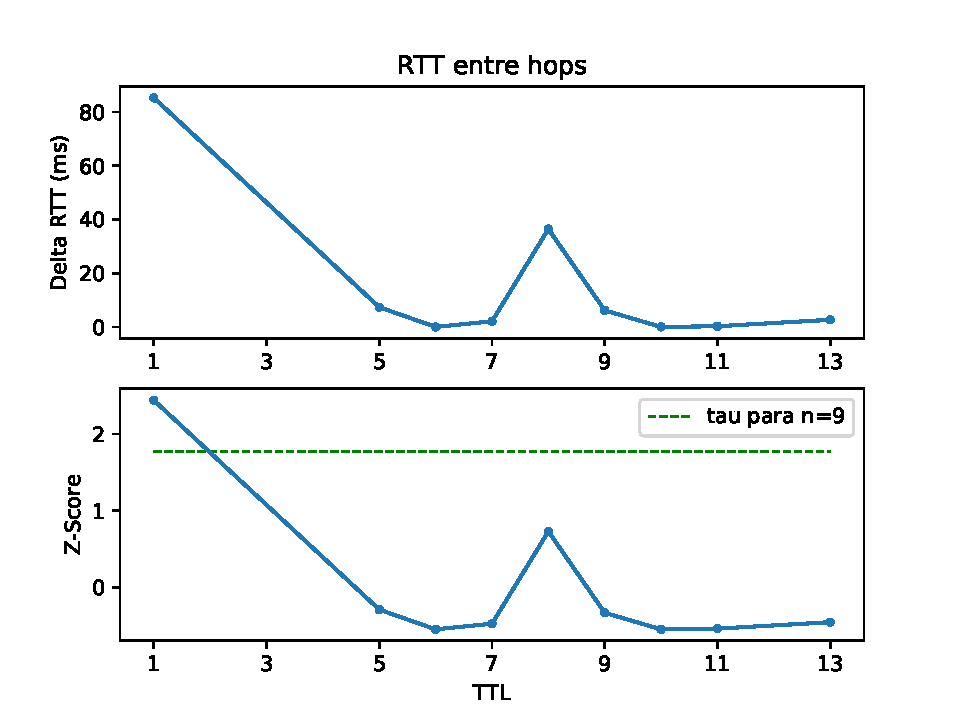
\includegraphics[width=8.5cm]{figs/traceroute-saopaulo.pdf}
  \caption{\normalfont RTT entre saltos (antes y después de normalizar respectivamente) para el sitio XXXXXXXXXXXXXXXXXXXXXX}
\end{figure}

Como se puede observar ... COMPLETAR.


\subsection*{Universidad de Sidney}

\subsubsection*{Recorrido en el Planisferio}

A continuación se puede ver de forma bastante clara como el paquete tuvo que pasar por estados unidos para luego ir a Europa Occidental hasta llegar finalmente a Rusia.

\begin{figure}[H]
  \centering
  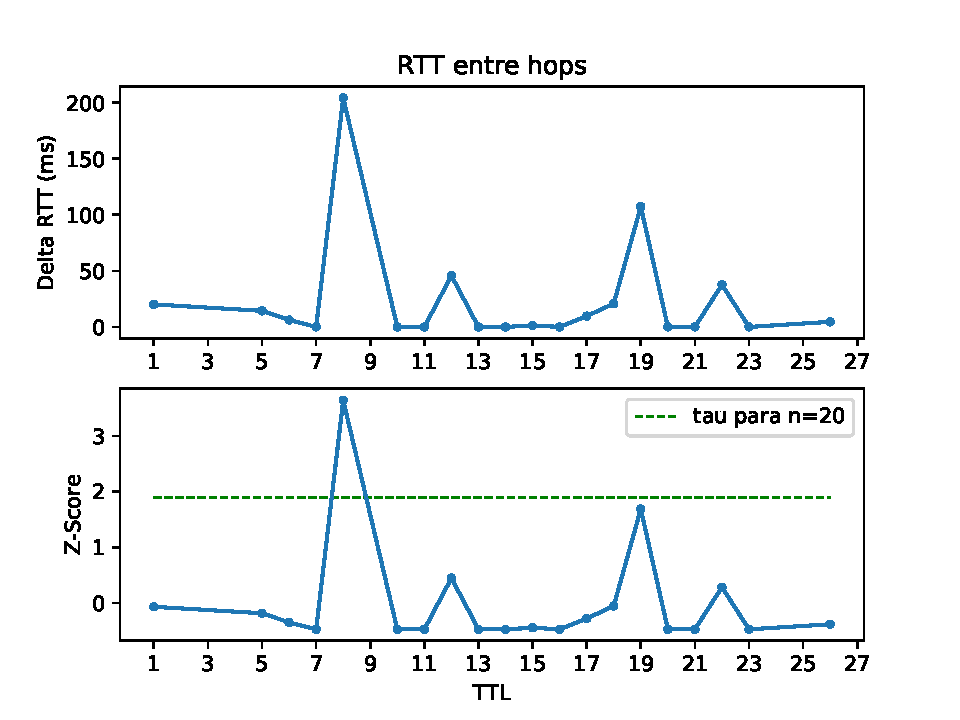
\includegraphics[width=8.5cm]{figs/traceroute-sidney.pdf}
  \caption{\normalfont Recorrido realizado por los paquetes durante la ejecución de traceroute al intentar alcanzar el sitio sydney.edu.au}
\end{figure}

\subsubsection*{RTT entre saltos}

A continuación intentamos ver los timepos entre saltos. Para esto calculamos la media de cada de los RTTs obtenidos de cada TTL para reducir a solo un valor las mediciones obtenidas por cada TTL. 

Seguido de esto realizamos dos experimentos. Primero simplemente restamos los RTTs medios entre si como se puede ver en el primer gráfico, luego llevamos el experimento un paso mas allá normalizando con z-score los RTTs para eliminar cualquier tipo de deformación en las dimensiones del gráfico.

\begin{figure}[H]
  \centering
  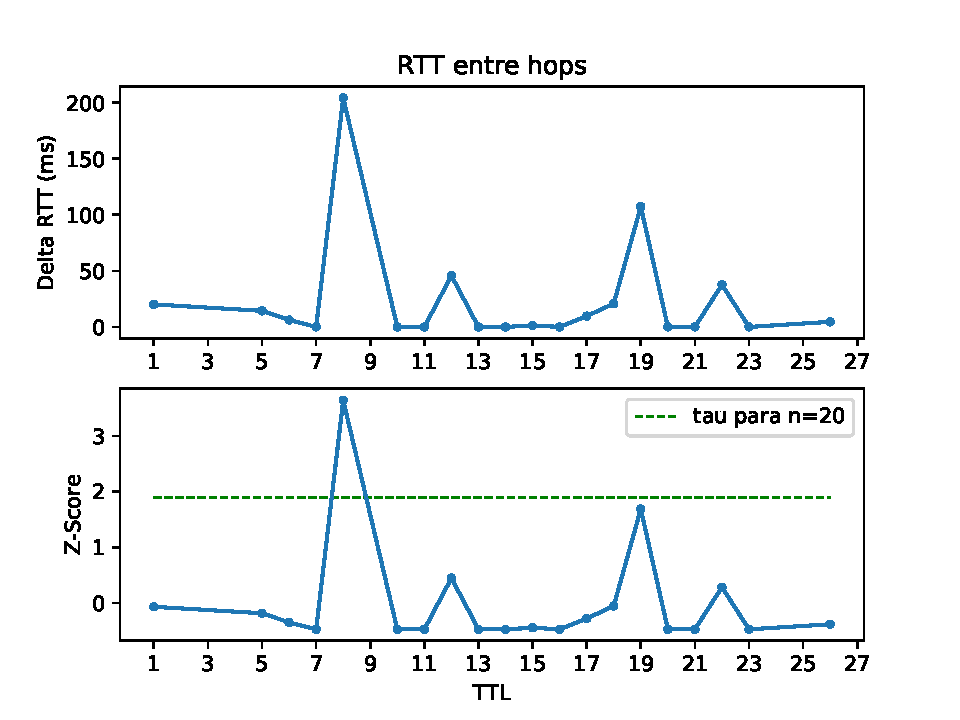
\includegraphics[width=8.5cm]{figs/traceroute-sidney.pdf}
  \caption{\normalfont RTT entre saltos (antes y después de normalizar respectivamente) para el sitio sydney.edu.au}
\end{figure}

Como se puede observar ... COMPLETAR.


\subsection*{Universidad de Moscow}

\subsubsection*{Recorrido en el Planisferio}

A continuación se puede ver de forma bastante clara como el paquete tuvo que pasar por estados unidos para luego ir a Europa Occidental hasta llegar finalmente a Rusia.

\begin{figure}[H]
  \centering
  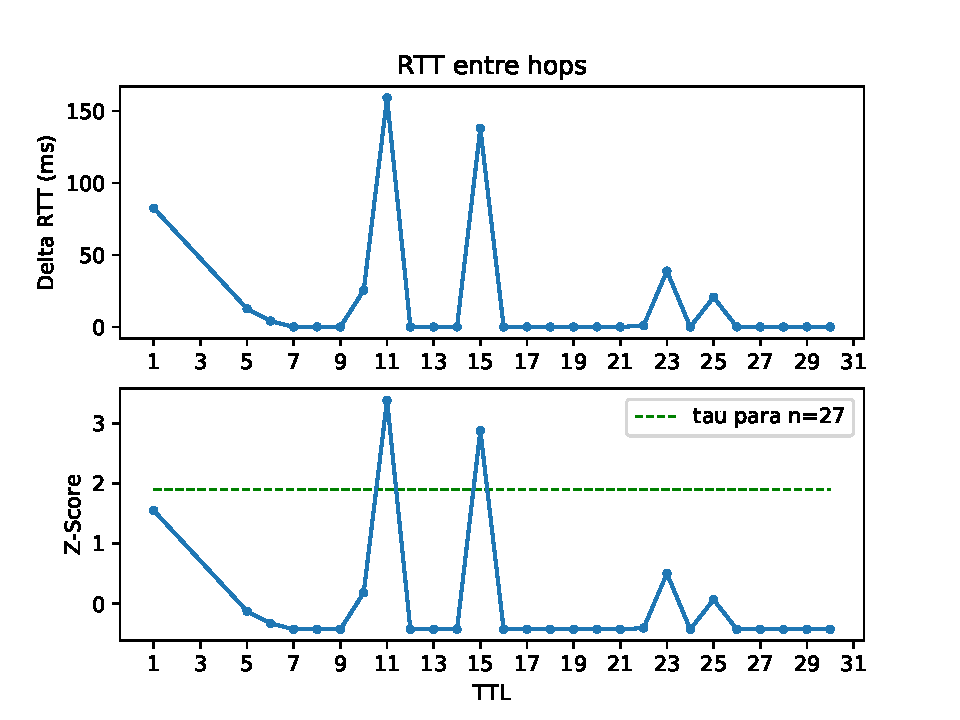
\includegraphics[width=8.5cm]{figs/traceroute-moscow.pdf}
  \caption{\normalfont Recorrido realizado por los paquetes durante la ejecución de traceroute al intentar alcanzar el sitio www.msu.com}
\end{figure}

\subsubsection*{RTT entre saltos}

A continuación intentamos ver los timepos entre saltos. Para esto calculamos la media de cada de los RTTs obtenidos de cada TTL para reducir a solo un valor las mediciones obtenidas por cada TTL. 

Seguido de esto realizamos dos experimentos. Primero simplemente restamos los RTTs medios entre si como se puede ver en el primer gráfico, luego llevamos el experimento un paso mas allá normalizando con z-score los RTTs para eliminar cualquier tipo de deformación en las dimensiones del gráfico.

\begin{figure}[H]
  \centering
  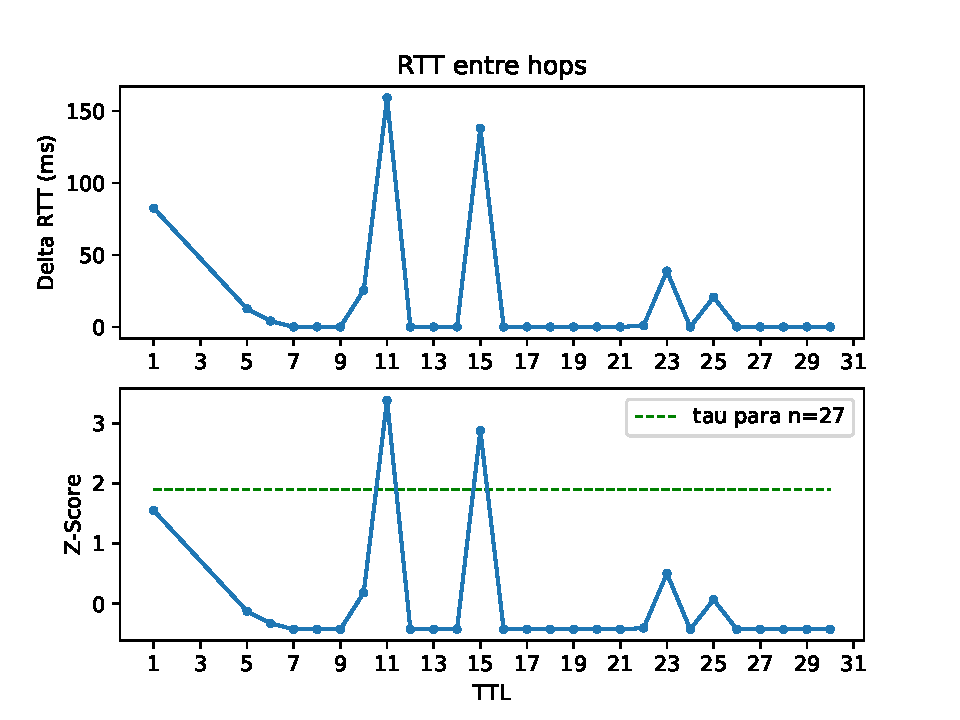
\includegraphics[width=8.5cm]{figs/traceroute-moscow.pdf}
  \caption{\normalfont RTT entre saltos (antes y después de normalizar respectivamente) para el sitio www.msu.com}
\end{figure}

Como se puede observar ... COMPLETAR.

\section{Discusión}

Recapitulando, de lo dicho hasta aquí nos llevamos las siguientes conclusiones:

\begin{itemize}
	\item Vimos, con el caso de Rusia, que este modelo es muy sensible a anomalías como los caminos asimétricos (que sospechamos que fue uno de los problemas), o las congestiones en la red (otra suposición). Este caso también ilustra una situación que no puede mejorarse con una valor de corte arbitrario (distinto de $\tau$) dado que los verdades saltos continentales tienen un RTT diferencial menor a los falsos.
	\item Aún en el caso de Australia, donde no parecieron verse anomalías grandes, el modelo tuvo problemas, infiriendo falsos enlaces continentales. El modelo parece demasiado simple para lidiar con la arbitrariedad de qué es y qué no un continente. Es notable que, por cómo funciona el método de Cimbala (ver un outlier a la vez, y sacarlo), aunque se detecten en forma correcta los enlaces continentales primero, luego quedan un set de puntos intracontinentales donde una gran distancia puede resultar un outlier (que no lo era si considerábamos el set completo). Esto hace que un caso como el de Australia, pueda terminar reduciéndose a varios como el de Brasil, encontrando falsos positivos. Posibles soluciones a esto serían tener siempre en consideración el \emph{big picture} de todos los puntos como parte del score. También podría devolverse la lista de outliers con un nivel de confianza sobre la posibilidad de que sean enlaces continentales o no. En definitiva, la influencia de la longitud de la ruta para el método actual es menor a lo que se esperaría.
	\item Entre un 10 y un 30 por ciento de los hops ignoraron la respuesta por time exceeded, esto nos llamó la atención ya que parece ser un número bastante alto, aunque investigando un poco descubrimos que este fenómeno no es para nada extraño. Las razones más comunes por lo que esto suele ocurrir parecen ser la configuración del hop para omitir la respuesta a estos mensajes y el bloqueo de paquetes desde el firewall según indica la documentación de traceroute \footnote{http://web.mit.edu/freebsd/head/contrib/traceroute/traceroute.c} y el artículo provisto por la cátedra \footnote{https://www.net.in.tum.de/fileadmin/TUM/NET/NET-2012-08-1/NET-2012-08-1\_02.pdf}.

\end{itemize}

En definitiva, notamos que este modelo tiene muchas oportunidades de mejora, y no es lo suficientemente robusto como para poder ser usado seriamente como un detector de enlaces intercontinentales. De hecho, salvo que se cuente con cierta metadata sobre el estado de la red, parece imposible tener un buen predictor, considerando la gran variedad de situaciones que se dan actualmente en las redes y que pueden meter ruido, desde congestiones hasta anomalías debidas a las topologías o los protocolos heterogéneos.


%----------------------------------------------------------------------

%\begin{thebibliography}{1}

%\bibitem{enunciado}
%C\'atedra de Teor\'ia de las Comunicaciones\\
%\newblock {\em Primer trabajo pr\'actico}\\
%\newblock Primer cuatrimestre $2013$

%\bibitem{arp}
%RFC 826 - Ethernet Address Resolution Protocol\\
%\url{http://tools.ietf.org/html/rfc826}\\
%\newblock C. Plummer $1982$

%\bibitem{conflicto}
%RFC 5227 - IPv4 Address Conflict Detection\\
%\url{http://tools.ietf.org/html/rfc3927}\\
%\newblock S. Cheshire $2008$

%\bibitem{link}
%RFC 3927 - Configuration of IPv4 Link-Local Addresses\\
%\url{http://tools.ietf.org/html/rfc3927}\\
%\newblock Cheshire, et al. $2005$

%\bibitem{patente}
%Method and apparatus for detecting a router that improperly responds to ARP requests\\
%\newblock US 7729292 B2\\
%\url{http://www.google.com/patents/US7729292}\\
%\newblock Stuart D. Cheshire y Joshua V. Graessley

%\bibitem{scapy}
%\texttt{Scapy}\\
%\url{http://www.secdev.org/projects/scapy}

%\bibitem{dhcp}
%RFC 1531 - Dynamic Host Configuration Protocol\\
%\url{https://tools.ietf.org/html/rfc1531}

%\bibitem{tcp}
%\url{http://www.tcpdump.org}

%\end{thebibliography}


\end{document}

